\newpage
\chapter*{Introduction}
\addcontentsline{toc}{chapter}{Introduction}

"Over the years \gls{Arduino} has been the brain of thousands of projects, from everyday objects to complex scientific instruments. A worldwide community of makers - students, hobbyists, artists, programmers, and professionals - has gathered around this open-source platform, their contributions have added up to an incredible amount of accessible knowledge that can be of great help to novices and experts alike."~\citep{arduino-15} 

%
\begin{figure}[ht]
	\centering
	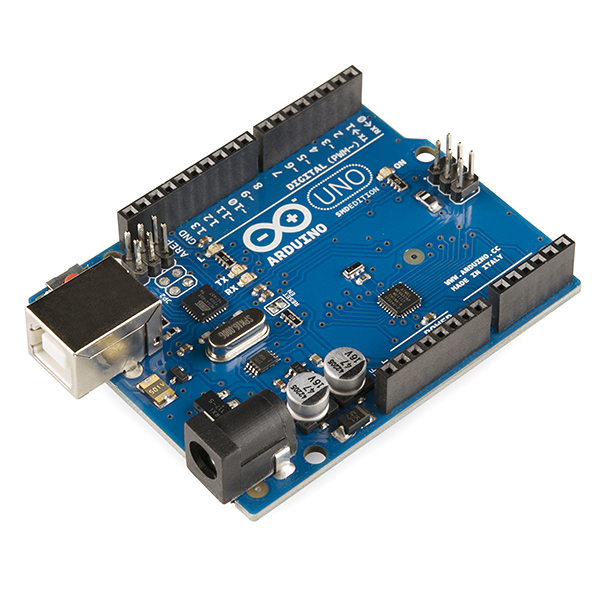
\includegraphics[width=8cm]{images/01}
	\caption{Arduino Uno R3 \citep{wikipedia-13}}
	\label{fig:arduino_uno_r3}
\end{figure}
%

\section*{Where might an Arduino be used?}
\addcontentsline{toc}{section}{Where might an Arduino be used?}
A few contrived examples of where one might use an Arduino in order to automate some process:

\subsection*{Automatic Dog's Water Bowl}
An dog owner wants to ensure her pet is never left without water. She attaches a system for measuring the water level in the dog's bowl. Her \gls{Arduino} is programmed to measure this value every 5 minutes. If this level falls below a certain value, a valve is opened and a water pump is activated to fill up the water bowl. It then sends an SMS to the owner to let her know that the dog is in safe hands.

\begin{itemize}
	\item Read inputs from a water level sensor
	\item Control a valve which lets water flow
	\item Control speed of a water pump 
	\item Send SMS to owner about giving the dog water
\end{itemize}


\subsection*{Bird Table Camera}
A rising social media ornithologist wishes to share pictures from all the visitors to the bird table in his garden. He mounts an infra-red movement sensor on the bird table attached to an \gls{Arduino} which is configured to record an image and send it to Twitter. His neighbours marvel at how many crows he's feeding.

\begin{itemize}
	\item Read inputs from a movement sensor
	\item Control a camera shutter
	\item Transmit image back to PC
	\item Send tweet with picture of the bird table visitor
\end{itemize}


\subsection*{Fingerprint Door Lock}
A student is sick of forgetting his keys and being locked out of his house. He uses a fingerprint scanner and an Arduino to make a biometric fingerprint door lock. He needs only scan his thumb print now and the door will unlock.

\begin{itemize}
	\item Read inputs from a fingerprint sensor
	\item Compares the finger print against an authorised fingerprint
	\item Records the time and date a finger was pressed on the scanner
	\item Makes audio error tone if the fingerprint was invalid
	\item If valid fingerprint it unlocks the door
\end{itemize}


\newpage
\section*{Workshop Aims}
\addcontentsline{toc}{section}{Workshop Aims}
In this workshop the aim is to give you a crash course in digital electronics, and providing you the basic skills to start using the Arduino micro-controllers in your future projects.

\begin{description}
	\item[Workshop Requirements] \hfill \\
	Each person will require the following:
	\begin{itemize}
		\item PC, either Linux, Mac or Windows can be used
		\item Arduino IDE pre-installed (Internet at the makerspace is flaky!)
		\item A sambo to keep you going
	\end{itemize}
	
	\item[Learning Outcomes] \hfill \\
	Each person will leave with:
	\begin{itemize}
		\item Arduino starter kit
		\item Crash course in digital electronics
		\item Confidence to use Arduino in future projects
	\end{itemize}
\end{description}

\subsection*{Arduino Starter Kit Contents}
The Arduino starter kit contains the following components, which we will be making use of during the workshop.

\begin{itemize}
	\item 1 $\times$ Arduino Compatible R3 Uno
	\item 1 $\times$ Breadboard
	\item 16 $\times$ jumper wires various colours
	\item 20 $\times$ 5mm LED's assorted colours
	\item 10 $\times$ 10k ohm resistors
	\item 10 $\times$ 330ohm resistors
	\item 1 $\times$ RGB LED
	\item 1 $\times$ photo resistor
	\item 2 $\times$ push buttons
	\item 1 $\times$ temperature sensor
	
\end{itemize}


\newpage
\section*{Basic Circuit Theory}
\addcontentsline{toc}{section}{Basic Circuit Theory}

In an electrical circuit there is a fundamental relationship between voltage, current and resistance and it is explained by Ohm’s Law~\citep{et-15}.

\subsection*{Voltage}
Voltage, (SI Unit: $V$ - Volts) is the potential energy of an electrical supply stored in the form of an electrical charge. Voltage can be thought of as the force that pushes electrons through a conductor and the greater the voltage the greater is its ability to push the electrons through a given circuit~\citep{et-15}.

%
\begin{figure}[ht]
	\centering
	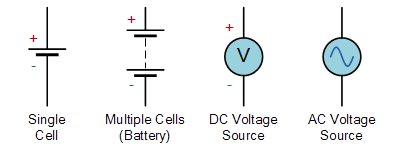
\includegraphics[width=7cm]{images/02}
	\caption{Voltage Symbols \citep{et-15}}
	\label{fig:voltage_symbols}
\end{figure}
%

\subsection*{Current}
Current, (SI Unit: $A$ - Ampere) is the movement or flow of electrical charge and is measured in Amperes. It is the continuous and uniform flow (called a drift) of electrons (the negative particles of an atom) around a circuit that are being pushed by the voltage source~\citep{et-15}.

%
\begin{figure}[ht]
	\centering
	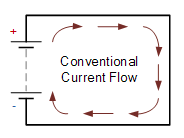
\includegraphics[width=4cm]{images/03}
	\caption{Current Symbols \citep{et-15}}
	\label{fig:current_symbols}
\end{figure}
%

\newpage
\subsection*{Resistance}
Resistance, (SI Unit: $\Omega$ - Ohms) of a circuit is its ability to resist or prevent the flow of current (electron flow) through itself making it necessary to apply a greater voltage to the electrical circuit to cause the current to flow again. Note that Resistance cannot be negative in value only positive~\citep{et-15}.

%
\begin{figure}[ht]
	\centering
	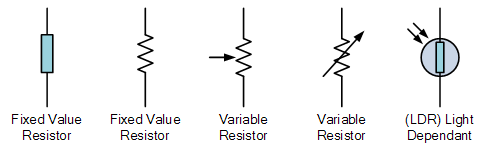
\includegraphics[width=8cm]{images/04}
	\caption{Resistance Symbols \citep{et-15}}
	\label{fig:resistance_symbols}
\end{figure}
%

\subsection*{Ohm's Law}
The following equation Ohm's Law explains the relationship between Voltage, Current and Resistance for an electrical circuit.

%
\begin{figure}[ht]
	\centering
	\begin{equation}
	V = I \times R
	\end{equation}
	\begin{equation}
	I = \frac{V}{R}
	\end{equation}
	\begin{equation}
	R = \frac{V}{I} 
	\end{equation}
	\caption{Ohm's Law}
	\label{fig:ohms_law_equation}
\end{figure}
%


\begin{itemize}
	\item Voltage, current \& resistance
	\item Ohms law
	\item Resistor, capacitor, LED, photo-resistor
	\item Breadboard
	\item Digital vs analogue signals
\end{itemize}


\section*{Basic Arduino Coding Concepts}
\addcontentsline{toc}{section}{Basic Arduino Coding Concepts}

\begin{itemize}
	\item Variables
	\item setup() function
	\item loop() function
\end{itemize}


\section*{Phenakistoscope Creation}
\addcontentsline{toc}{section}{Phenakistoscope Creation}


\citep{kalif-15-a} \citep{kalif-15-b}


%
\begin{table}
	\centering
	\begin{tabular}{p{4cm} l}
		\toprule
		Column 1 & Column 2\\ \midrule
		x & 1 \\
		y & 2 \\
		z & 3 \\
		\bottomrule
	\end{tabular}
	\caption{Table Caption}
	\label{tab:table_label}
\end{table}
%